\documentclass[]{article}
\usepackage{lmodern}
\usepackage{amssymb,amsmath}
\usepackage{ifxetex,ifluatex}
\usepackage{fixltx2e} % provides \textsubscript
\ifnum 0\ifxetex 1\fi\ifluatex 1\fi=0 % if pdftex
  \usepackage[T1]{fontenc}
  \usepackage[utf8]{inputenc}
\else % if luatex or xelatex
  \ifxetex
    \usepackage{mathspec}
  \else
    \usepackage{fontspec}
  \fi
  \defaultfontfeatures{Ligatures=TeX,Scale=MatchLowercase}
\fi
% use upquote if available, for straight quotes in verbatim environments
\IfFileExists{upquote.sty}{\usepackage{upquote}}{}
% use microtype if available
\IfFileExists{microtype.sty}{%
\usepackage{microtype}
\UseMicrotypeSet[protrusion]{basicmath} % disable protrusion for tt fonts
}{}
\usepackage[margin=1in]{geometry}
\usepackage{hyperref}
\hypersetup{unicode=true,
            pdfborder={0 0 0},
            breaklinks=true}
\urlstyle{same}  % don't use monospace font for urls
\usepackage{color}
\usepackage{fancyvrb}
\newcommand{\VerbBar}{|}
\newcommand{\VERB}{\Verb[commandchars=\\\{\}]}
\DefineVerbatimEnvironment{Highlighting}{Verbatim}{commandchars=\\\{\}}
% Add ',fontsize=\small' for more characters per line
\usepackage{framed}
\definecolor{shadecolor}{RGB}{248,248,248}
\newenvironment{Shaded}{\begin{snugshade}}{\end{snugshade}}
\newcommand{\KeywordTok}[1]{\textcolor[rgb]{0.13,0.29,0.53}{\textbf{#1}}}
\newcommand{\DataTypeTok}[1]{\textcolor[rgb]{0.13,0.29,0.53}{#1}}
\newcommand{\DecValTok}[1]{\textcolor[rgb]{0.00,0.00,0.81}{#1}}
\newcommand{\BaseNTok}[1]{\textcolor[rgb]{0.00,0.00,0.81}{#1}}
\newcommand{\FloatTok}[1]{\textcolor[rgb]{0.00,0.00,0.81}{#1}}
\newcommand{\ConstantTok}[1]{\textcolor[rgb]{0.00,0.00,0.00}{#1}}
\newcommand{\CharTok}[1]{\textcolor[rgb]{0.31,0.60,0.02}{#1}}
\newcommand{\SpecialCharTok}[1]{\textcolor[rgb]{0.00,0.00,0.00}{#1}}
\newcommand{\StringTok}[1]{\textcolor[rgb]{0.31,0.60,0.02}{#1}}
\newcommand{\VerbatimStringTok}[1]{\textcolor[rgb]{0.31,0.60,0.02}{#1}}
\newcommand{\SpecialStringTok}[1]{\textcolor[rgb]{0.31,0.60,0.02}{#1}}
\newcommand{\ImportTok}[1]{#1}
\newcommand{\CommentTok}[1]{\textcolor[rgb]{0.56,0.35,0.01}{\textit{#1}}}
\newcommand{\DocumentationTok}[1]{\textcolor[rgb]{0.56,0.35,0.01}{\textbf{\textit{#1}}}}
\newcommand{\AnnotationTok}[1]{\textcolor[rgb]{0.56,0.35,0.01}{\textbf{\textit{#1}}}}
\newcommand{\CommentVarTok}[1]{\textcolor[rgb]{0.56,0.35,0.01}{\textbf{\textit{#1}}}}
\newcommand{\OtherTok}[1]{\textcolor[rgb]{0.56,0.35,0.01}{#1}}
\newcommand{\FunctionTok}[1]{\textcolor[rgb]{0.00,0.00,0.00}{#1}}
\newcommand{\VariableTok}[1]{\textcolor[rgb]{0.00,0.00,0.00}{#1}}
\newcommand{\ControlFlowTok}[1]{\textcolor[rgb]{0.13,0.29,0.53}{\textbf{#1}}}
\newcommand{\OperatorTok}[1]{\textcolor[rgb]{0.81,0.36,0.00}{\textbf{#1}}}
\newcommand{\BuiltInTok}[1]{#1}
\newcommand{\ExtensionTok}[1]{#1}
\newcommand{\PreprocessorTok}[1]{\textcolor[rgb]{0.56,0.35,0.01}{\textit{#1}}}
\newcommand{\AttributeTok}[1]{\textcolor[rgb]{0.77,0.63,0.00}{#1}}
\newcommand{\RegionMarkerTok}[1]{#1}
\newcommand{\InformationTok}[1]{\textcolor[rgb]{0.56,0.35,0.01}{\textbf{\textit{#1}}}}
\newcommand{\WarningTok}[1]{\textcolor[rgb]{0.56,0.35,0.01}{\textbf{\textit{#1}}}}
\newcommand{\AlertTok}[1]{\textcolor[rgb]{0.94,0.16,0.16}{#1}}
\newcommand{\ErrorTok}[1]{\textcolor[rgb]{0.64,0.00,0.00}{\textbf{#1}}}
\newcommand{\NormalTok}[1]{#1}
\usepackage{graphicx,grffile}
\makeatletter
\def\maxwidth{\ifdim\Gin@nat@width>\linewidth\linewidth\else\Gin@nat@width\fi}
\def\maxheight{\ifdim\Gin@nat@height>\textheight\textheight\else\Gin@nat@height\fi}
\makeatother
% Scale images if necessary, so that they will not overflow the page
% margins by default, and it is still possible to overwrite the defaults
% using explicit options in \includegraphics[width, height, ...]{}
\setkeys{Gin}{width=\maxwidth,height=\maxheight,keepaspectratio}
\IfFileExists{parskip.sty}{%
\usepackage{parskip}
}{% else
\setlength{\parindent}{0pt}
\setlength{\parskip}{6pt plus 2pt minus 1pt}
}
\setlength{\emergencystretch}{3em}  % prevent overfull lines
\providecommand{\tightlist}{%
  \setlength{\itemsep}{0pt}\setlength{\parskip}{0pt}}
\setcounter{secnumdepth}{0}
% Redefines (sub)paragraphs to behave more like sections
\ifx\paragraph\undefined\else
\let\oldparagraph\paragraph
\renewcommand{\paragraph}[1]{\oldparagraph{#1}\mbox{}}
\fi
\ifx\subparagraph\undefined\else
\let\oldsubparagraph\subparagraph
\renewcommand{\subparagraph}[1]{\oldsubparagraph{#1}\mbox{}}
\fi

%%% Use protect on footnotes to avoid problems with footnotes in titles
\let\rmarkdownfootnote\footnote%
\def\footnote{\protect\rmarkdownfootnote}

%%% Change title format to be more compact
\usepackage{titling}

% Create subtitle command for use in maketitle
\newcommand{\subtitle}[1]{
  \posttitle{
    \begin{center}\large#1\end{center}
    }
}

\setlength{\droptitle}{-2em}
  \title{}
  \pretitle{\vspace{\droptitle}}
  \posttitle{}
  \author{}
  \preauthor{}\postauthor{}
  \date{}
  \predate{}\postdate{}


\begin{document}

\section{The Dynamic-p Technique with
lavaan}\label{the-dynamic-p-technique-with-lavaan}

The purpose of this project is to demonstrate how to fit a
single-subject structural equation model within the dynamic p-technique
framework. As discussed in the primary manuscript, of the recent
introductions to and tutorials on the dynamic p-technique, we believe
the method outlined in Little's (2013) text is the most thorough and
approachable for non-statistician behavioral researchers. Thus, the
approach described herein is based primarily on Little's text.
Longitudinal structural equation models, such as those estimated with
the dynamic p-technique, can become very complex.

First we'll load the data and open our first two packages.

\begin{Shaded}
\begin{Highlighting}[]
\KeywordTok{library}\NormalTok{(readxl)}
\KeywordTok{library}\NormalTok{(tidyverse)}

\NormalTok{d <-}\StringTok{ }\KeywordTok{read_excel}\NormalTok{(}\StringTok{"Lindsey.xlsx"}\NormalTok{)}

\KeywordTok{glimpse}\NormalTok{(d)}
\end{Highlighting}
\end{Shaded}

\begin{verbatim}
## Observations: 103
## Variables: 9
## $ Date <dttm> 2016-01-29, 2016-01-30, 2016-01-31, 2016-02-01, 2016-02-02, 2016-02-03, 2016-02-0...
## $ Meds <dbl> 1, NA, NA, NA, 1, 1, 1, NA, NA, 0, 1, 1, 1, 1, NA, 0, 1, 1, 1, 1, 1, 1, NA, 0, 1, ...
## $ A3   <dbl> 3, NA, NA, NA, 4, 3, 5, NA, NA, 4, 3, 3, 3, 4, NA, 4, 3, 4, 3, 2, 3, 2, NA, 4, 4, ...
## $ A8   <dbl> 3, NA, NA, NA, 2, 4, 5, NA, NA, 4, 3, 4, 4, 4, NA, 5, 4, 4, 4, 4, 4, 2, NA, 3, 4, ...
## $ A10  <dbl> 5, NA, NA, NA, 3, 5, 3, NA, NA, 3, 4, 3, 4, 3, NA, 4, 3, 5, 3, 2, 3, 2, NA, 4, 5, ...
## $ A13  <dbl> 4, NA, NA, NA, 5, 4, 4, NA, NA, 2, 4, 4, 3, 3, NA, 1, 4, 5, 5, 2, 3, 2, NA, 2, 5, ...
## $ A14  <dbl> 5, NA, NA, NA, 4, 5, 4, NA, NA, 3, 4, 4, 4, 3, NA, 2, 4, 5, 5, 3, 3, 2, NA, 3, 5, ...
## $ A16  <dbl> 3, NA, NA, NA, 2, 1, 1, NA, NA, 2, 2, 2, 2, 2, NA, 1, 2, 2, 3, 2, 1, 1, NA, 1, 4, ...
## $ A17  <dbl> 3, NA, NA, NA, 1, 2, 3, NA, NA, 1, 3, 3, 4, 3, NA, 4, 3, 4, 3, 2, 3, 2, NA, 3, 5, ...
\end{verbatim}

In this document, we'll use functions and syntax from the
\href{https://www.tidyverse.org}{tidyverse}, which you might learn about
\href{http://r4ds.had.co.nz/transform.html}{here} or
\href{http://style.tidyverse.org}{here}.

Note how the data are in the long format. That is, although we have one
participant, ``Lindsey'', her data are presented in 103 rows, each
corresponding to a different calendar day.

\subsection{Descriptive statistics}\label{descriptive-statistics}

If you wanted to get a sense of the distributions of the ASRS items,
histograms might be handy.

\begin{Shaded}
\begin{Highlighting}[]
\NormalTok{d }\OperatorTok\StringTok{ }
\StringTok{  }\KeywordTok{select}\NormalTok{(A3}\OperatorTok{:}\NormalTok{A17) }\OperatorTok\StringTok{ }
\StringTok{  }\KeywordTok{gather}\NormalTok{(item, rating) }\OperatorTok\StringTok{ }
\StringTok{  }
\StringTok{  }\KeywordTok{ggplot}\NormalTok{(}\KeywordTok{aes}\NormalTok{(}\DataTypeTok{x =}\NormalTok{ rating)) }\OperatorTok{+}
\StringTok{  }\KeywordTok{geom_histogram}\NormalTok{(}\DataTypeTok{binwidth =} \DecValTok{1}\NormalTok{, }\DataTypeTok{fill =} \StringTok{"chartreuse2"}\NormalTok{, }\DataTypeTok{color =} \StringTok{"grey92"}\NormalTok{, }\DataTypeTok{size =} \DecValTok{1}\OperatorTok{/}\DecValTok{5}\NormalTok{) }\OperatorTok{+}
\StringTok{  }\KeywordTok{theme}\NormalTok{(}\DataTypeTok{panel.grid =} \KeywordTok{element_blank}\NormalTok{()) }\OperatorTok{+}
\StringTok{  }\KeywordTok{facet_wrap}\NormalTok{(}\OperatorTok{~}\NormalTok{item, }\DataTypeTok{ncol =} \DecValTok{4}\NormalTok{)}
\end{Highlighting}
\end{Shaded}

\begin{verbatim}
## Warning: Removed 112 rows containing non-finite values (stat_bin).
\end{verbatim}

\includegraphics{README_files/figure-latex/unnamed-chunk-2-1.pdf}

Happily, their distributions look reasonable. You can get a sense of
their values over time with a sequentially-color-coded tile plot.

\begin{Shaded}
\begin{Highlighting}[]
\KeywordTok{library}\NormalTok{(viridis)}

\NormalTok{d }\OperatorTok\StringTok{ }
\StringTok{  }\KeywordTok{select}\NormalTok{(Date, A3}\OperatorTok{:}\NormalTok{A17) }\OperatorTok\StringTok{ }
\StringTok{  }\KeywordTok{gather}\NormalTok{(item, rating, }\OperatorTok{-}\NormalTok{Date) }\OperatorTok
\StringTok{  }\KeywordTok{mutate}\NormalTok{(}\DataTypeTok{rating =} \KeywordTok{factor}\NormalTok{(rating, }\DataTypeTok{levels =} \KeywordTok{c}\NormalTok{(}\DecValTok{1}\OperatorTok{:}\DecValTok{5}\NormalTok{)),}
         \DataTypeTok{item =} \KeywordTok{factor}\NormalTok{(item, }\DataTypeTok{levels =} \KeywordTok{c}\NormalTok{(}\StringTok{"A3"}\NormalTok{, }\StringTok{"A8"}\NormalTok{, }\StringTok{"A10"}\NormalTok{, }\StringTok{"A13"}\NormalTok{, }\StringTok{"A14"}\NormalTok{, }\StringTok{"A16"}\NormalTok{, }\StringTok{"A17"}\NormalTok{))) }\OperatorTok\StringTok{ }
\StringTok{  }
\StringTok{  }\KeywordTok{ggplot}\NormalTok{(}\KeywordTok{aes}\NormalTok{(}\DataTypeTok{x =}\NormalTok{ Date, }\DataTypeTok{y =}\NormalTok{ item)) }\OperatorTok{+}
\StringTok{  }\KeywordTok{geom_raster}\NormalTok{(}\KeywordTok{aes}\NormalTok{(}\DataTypeTok{fill =}\NormalTok{ rating)) }\OperatorTok{+}
\StringTok{  }\KeywordTok{scale_fill_viridis}\NormalTok{(}\OtherTok{NULL}\NormalTok{, }\DataTypeTok{discrete =} \OtherTok{TRUE}\NormalTok{, }\DataTypeTok{option =} \StringTok{"D"}\NormalTok{,}
                     \DataTypeTok{guide =} \KeywordTok{guide_legend}\NormalTok{(}\DataTypeTok{direction =} \StringTok{"horizontal"}\NormalTok{,}
                                          \DataTypeTok{nrow =} \DecValTok{1}\NormalTok{)) }\OperatorTok{+}
\StringTok{  }\KeywordTok{scale_x_datetime}\NormalTok{(}\DataTypeTok{expand =} \KeywordTok{c}\NormalTok{(}\DecValTok{0}\NormalTok{, }\DecValTok{0}\NormalTok{)) }\OperatorTok{+}
\StringTok{  }\KeywordTok{scale_y_discrete}\NormalTok{(}\DataTypeTok{expand =} \KeywordTok{c}\NormalTok{(}\DecValTok{0}\NormalTok{, }\DecValTok{0}\NormalTok{)) }\OperatorTok{+}
\StringTok{  }\KeywordTok{labs}\NormalTok{(}\DataTypeTok{x =} \OtherTok{NULL}\NormalTok{, }\DataTypeTok{y =} \OtherTok{NULL}\NormalTok{) }\OperatorTok{+}
\StringTok{  }\KeywordTok{theme}\NormalTok{(}\DataTypeTok{panel.grid =} \KeywordTok{element_blank}\NormalTok{(),}
        \DataTypeTok{axis.text.y =} \KeywordTok{element_text}\NormalTok{(}\DataTypeTok{hjust =} \DecValTok{0}\NormalTok{),}
        \DataTypeTok{axis.ticks.y =} \KeywordTok{element_blank}\NormalTok{(),}
        \DataTypeTok{legend.position =} \StringTok{"top"}\NormalTok{)}
\end{Highlighting}
\end{Shaded}

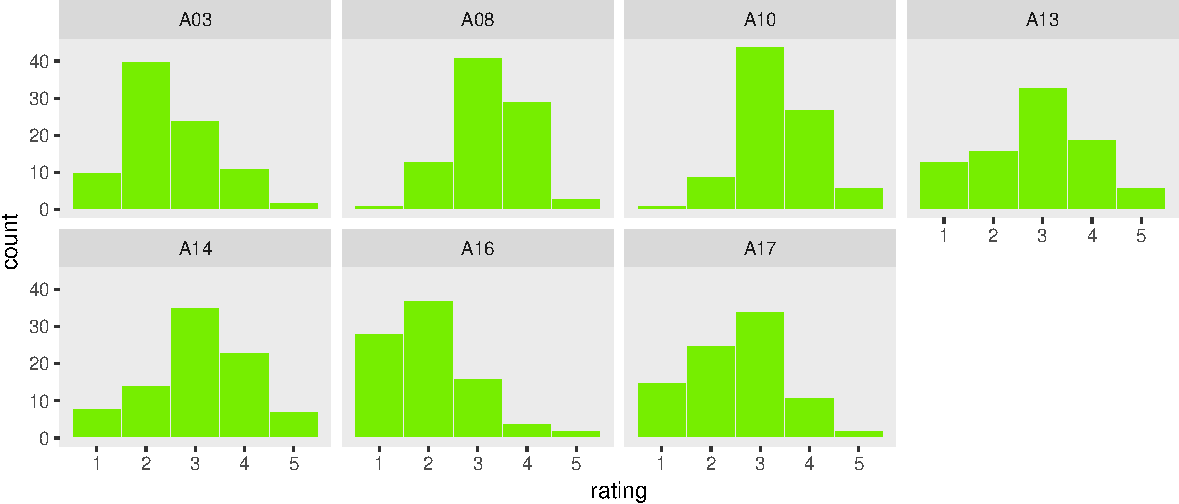
\includegraphics{README_files/figure-latex/unnamed-chunk-3-1.pdf}

And with the
\href{https://cran.r-project.org/web/packages/psych/index.html}{psych
package}, we can use the \texttt{describe()} function to get the typical
descriptive statistics.

\begin{Shaded}
\begin{Highlighting}[]
\KeywordTok{library}\NormalTok{(psych)}

\NormalTok{d }\OperatorTok\StringTok{ }
\StringTok{  }\KeywordTok{select}\NormalTok{(A3}\OperatorTok{:}\NormalTok{A17) }\OperatorTok\StringTok{ }
\StringTok{  }\KeywordTok{describe}\NormalTok{()}
\end{Highlighting}
\end{Shaded}

\begin{verbatim}
##     vars  n mean   sd median trimmed  mad min max range  skew kurtosis   se
## A3     1 87 2.48 0.94      2    2.45 1.48   1   5     4  0.51    -0.17 0.10
## A8     2 87 3.23 0.79      3    3.25 1.48   1   5     4 -0.14    -0.19 0.08
## A10    3 87 3.32 0.80      3    3.32 0.00   1   5     4  0.05     0.10 0.09
## A13    4 87 2.87 1.13      3    2.87 1.48   1   5     4 -0.09    -0.72 0.12
## A14    5 87 3.08 1.06      3    3.11 1.48   1   5     4 -0.22    -0.44 0.11
## A16    6 87 2.02 0.95      2    1.92 1.48   1   5     4  0.91     0.69 0.10
## A17    7 87 2.54 1.00      3    2.52 1.48   1   5     4  0.10    -0.55 0.11
\end{verbatim}

Recall that the items in the ASRS correspond to the 18 criterion A
symptoms, with the first nine classified as Inattentive and the last
nine as hyperactive/impulsive. For the sake of this example, we'll focus
on Lindsey's hyperactive/impulsive symptoms, ASRS items 10, 13, 14, 16,
and 17. The following code drops the other two, items 3 and 8.

\begin{Shaded}
\begin{Highlighting}[]
\NormalTok{d <-}
\StringTok{  }\NormalTok{d }\OperatorTok\StringTok{ }
\StringTok{  }\KeywordTok{select}\NormalTok{(}\KeywordTok{everything}\NormalTok{(), }\OperatorTok{-}\NormalTok{A3, }\OperatorTok{-}\NormalTok{A8)}
\end{Highlighting}
\end{Shaded}

\subsection{P-technique CFA}\label{p-technique-cfa}

Here we open our primary statistical package,
\href{https://cran.r-project.org/web/packages/lavaan/index.html}{lavaan},
which you might learn more about
\href{https://dornsife.usc.edu/assets/sites/210/docs/GC3/lavaan_tutorial.pdf}{here}
or \href{http://lavaan.ugent.be/tutorial/index.html}{here}.

\begin{Shaded}
\begin{Highlighting}[]
\KeywordTok{library}\NormalTok{(lavaan)}
\end{Highlighting}
\end{Shaded}

\subsubsection{0-lag.}\label{lag.}

The simplest starting place is a p-technique factor analysis. Using this
approach, the model syntax looks much like that of a typical group-level
CFA.

\begin{Shaded}
\begin{Highlighting}[]
\NormalTok{CFA_0_lag <-}\StringTok{ '}
\StringTok{H =~ NA*A10 + A13 + A14 + A16 + A17}

\StringTok{# Standardize the variance}
\StringTok{H ~~ 1*H}
\StringTok{'}
\end{Highlighting}
\end{Shaded}

Here we fit the model.

\begin{Shaded}
\begin{Highlighting}[]
\NormalTok{fit.CFA_0_lag <-}\StringTok{ }
\StringTok{  }\KeywordTok{cfa}\NormalTok{(CFA_0_lag, }
      \DataTypeTok{data =}\NormalTok{ d,}
      \DataTypeTok{estimator =} \StringTok{"MLR"}\NormalTok{,}
      \DataTypeTok{missing =} \StringTok{"ML"}\NormalTok{)}
\end{Highlighting}
\end{Shaded}

\begin{verbatim}
## Warning in lav_data_full(data = data, group = group, cluster = cluster, : lavaan WARNING: some cases are empty and will be ignored:
##   2 3 4 8 9 15 23 26 29 30 51 57 69 72 79 86
\end{verbatim}

The summary, including the typical fit indices and 95\% CIs for good
measure:

\begin{Shaded}
\begin{Highlighting}[]
\KeywordTok{summary}\NormalTok{(fit.CFA_0_lag, }
        \DataTypeTok{fit.measures =}\NormalTok{ T,}
        \DataTypeTok{ci =}\NormalTok{ T)}
\end{Highlighting}
\end{Shaded}

\begin{verbatim}
## lavaan (0.5-23.1097) converged normally after  18 iterations
## 
##                                                   Used       Total
##   Number of observations                            87         103
## 
##   Number of missing patterns                         1
## 
##   Estimator                                         ML      Robust
##   Minimum Function Test Statistic                7.452       6.768
##   Degrees of freedom                                 5           5
##   P-value (Chi-square)                           0.189       0.238
##   Scaling correction factor                                  1.101
##     for the Yuan-Bentler correction
## 
## Model test baseline model:
## 
##   Minimum Function Test Statistic              123.262     105.281
##   Degrees of freedom                                10          10
##   P-value                                        0.000       0.000
## 
## User model versus baseline model:
## 
##   Comparative Fit Index (CFI)                    0.978       0.981
##   Tucker-Lewis Index (TLI)                       0.957       0.963
## 
##   Robust Comparative Fit Index (CFI)                         0.983
##   Robust Tucker-Lewis Index (TLI)                            0.965
## 
## Loglikelihood and Information Criteria:
## 
##   Loglikelihood user model (H0)               -548.428    -548.428
##   Scaling correction factor                                  1.061
##     for the MLR correction
##   Loglikelihood unrestricted model (H1)       -544.702    -544.702
##   Scaling correction factor                                  1.071
##     for the MLR correction
## 
##   Number of free parameters                         15          15
##   Akaike (AIC)                                1126.856    1126.856
##   Bayesian (BIC)                              1163.845    1163.845
##   Sample-size adjusted Bayesian (BIC)         1116.515    1116.515
## 
## Root Mean Square Error of Approximation:
## 
##   RMSEA                                          0.075       0.064
##   90 Percent Confidence Interval          0.000  0.179       0.000  0.167
##   P-value RMSEA <= 0.05                          0.295       0.354
## 
##   Robust RMSEA                                               0.067
##   90 Percent Confidence Interval                             0.000  0.180
## 
## Standardized Root Mean Square Residual:
## 
##   SRMR                                           0.049       0.049
## 
## Parameter Estimates:
## 
##   Information                                 Observed
##   Standard Errors                   Robust.huber.white
## 
## Latent Variables:
##                    Estimate  Std.Err  z-value  P(>|z|) ci.lower ci.upper
##   H =~                                                                  
##     A10               0.222    0.099    2.237    0.025    0.027    0.417
##     A13               1.063    0.104   10.252    0.000    0.860    1.266
##     A14               0.885    0.102    8.659    0.000    0.684    1.085
##     A16               0.056    0.107    0.523    0.601   -0.153    0.265
##     A17               0.488    0.107    4.574    0.000    0.279    0.697
## 
## Intercepts:
##                    Estimate  Std.Err  z-value  P(>|z|) ci.lower ci.upper
##    .A10               3.322    0.085   38.973    0.000    3.155    3.489
##    .A13               2.874    0.120   23.879    0.000    2.638    3.109
##    .A14               3.080    0.113   27.291    0.000    2.859    3.302
##    .A16               2.023    0.101   19.934    0.000    1.824    2.222
##    .A17               2.540    0.106   23.885    0.000    2.332    2.749
##     H                 0.000                               0.000    0.000
## 
## Variances:
##                    Estimate  Std.Err  z-value  P(>|z|) ci.lower ci.upper
##     H                 1.000                               1.000    1.000
##    .A10               0.583    0.088    6.591    0.000    0.409    0.756
##    .A13               0.130    0.163    0.799    0.424   -0.189    0.449
##    .A14               0.326    0.126    2.577    0.010    0.078    0.574
##    .A16               0.893    0.162    5.498    0.000    0.575    1.211
##    .A17               0.746    0.126    5.929    0.000    0.500    0.993
\end{verbatim}

\subsubsection{1-lag.}\label{lag.-1}

\paragraph{First, we need to process the data a
bit.}\label{first-we-need-to-process-the-data-a-bit.}

Before we proceed to fit a dynamic-p CFA, we'll need to lag our data
file. In short, a lag is the difference from one measuremet occasion to
another. Since these are daily-diary data, each lag is a day in
separation.

Before we lag the data file, we'll add a row to the end of the data.
Because this row corresponds to \texttt{Date\ =\ "2016-05-11"}, a day
for which we don't have any information other than it was a Wednesday,
we'll insert NAs into most of the columns.

\begin{Shaded}
\begin{Highlighting}[]
\KeywordTok{tail}\NormalTok{(d)}
\end{Highlighting}
\end{Shaded}

\begin{verbatim}
## # A tibble: 6 x 7
##   Date                 Meds   A10   A13   A14   A16   A17
##   <dttm>              <dbl> <dbl> <dbl> <dbl> <dbl> <dbl>
## 1 2016-05-05 00:00:00  1.00  4.00  3.00  3.00  1.00  4.00
## 2 2016-05-06 00:00:00  1.00  3.00  2.00  3.00  2.00  1.00
## 3 2016-05-07 00:00:00  0     3.00  1.00  1.00  2.00  1.00
## 4 2016-05-08 00:00:00  1.00  2.00  2.00  3.00  3.00  1.00
## 5 2016-05-09 00:00:00  1.00  3.00  3.00  3.00  1.00  1.00
## 6 2016-05-10 00:00:00  1.00  2.00  3.00  4.00  1.00  1.00
\end{verbatim}

\begin{Shaded}
\begin{Highlighting}[]
\NormalTok{d_lagged <-}
\StringTok{  }\NormalTok{d }\OperatorTok\StringTok{ }
\StringTok{  }\KeywordTok{add_row}\NormalTok{(., }\DataTypeTok{Date =} \StringTok{"2016-05-11 00:00:00"}\NormalTok{, }
          \DataTypeTok{Meds =} \OtherTok{NA}\NormalTok{, }
          \DataTypeTok{A10 =} \OtherTok{NA}\NormalTok{, }\DataTypeTok{A13 =} \OtherTok{NA}\NormalTok{, }\DataTypeTok{A14 =} \OtherTok{NA}\NormalTok{, }\DataTypeTok{A16 =} \OtherTok{NA}\NormalTok{, }\DataTypeTok{A17 =} \OtherTok{NA}\NormalTok{)}
\end{Highlighting}
\end{Shaded}

With the \texttt{lag()} function, we'll add lagged values for our
\texttt{Meds} dummy and our ASRS items. For each of the lagged columns,
we'll add the suffix \texttt{\_1} to help differentiate them from the
original columns.

\begin{Shaded}
\begin{Highlighting}[]
\NormalTok{(}
\NormalTok{  d_lagged <-}
\StringTok{  }\NormalTok{d_lagged }\OperatorTok\StringTok{ }
\StringTok{  }\KeywordTok{mutate}\NormalTok{(}\DataTypeTok{Meds_1 =} \KeywordTok{lag}\NormalTok{(Meds),}
         \DataTypeTok{A10_1  =} \KeywordTok{lag}\NormalTok{(A10),}
         \DataTypeTok{A13_1  =} \KeywordTok{lag}\NormalTok{(A13),}
         \DataTypeTok{A14_1  =} \KeywordTok{lag}\NormalTok{(A14),}
         \DataTypeTok{A16_1  =} \KeywordTok{lag}\NormalTok{(A16),}
         \DataTypeTok{A17_1  =} \KeywordTok{lag}\NormalTok{(A17))}
\NormalTok{  )}
\end{Highlighting}
\end{Shaded}

\begin{verbatim}
## # A tibble: 104 x 13
##    Date                 Meds   A10   A13   A14   A16   A17 Meds_1 A10_1 A13_1 A14_1 A16_1 A17_1
##    <dttm>              <dbl> <dbl> <dbl> <dbl> <dbl> <dbl>  <dbl> <dbl> <dbl> <dbl> <dbl> <dbl>
##  1 2016-01-29 00:00:00  1.00  5.00  4.00  5.00  3.00  3.00  NA    NA    NA    NA    NA    NA   
##  2 2016-01-30 00:00:00 NA    NA    NA    NA    NA    NA      1.00  5.00  4.00  5.00  3.00  3.00
##  3 2016-01-31 00:00:00 NA    NA    NA    NA    NA    NA     NA    NA    NA    NA    NA    NA   
##  4 2016-02-01 00:00:00 NA    NA    NA    NA    NA    NA     NA    NA    NA    NA    NA    NA   
##  5 2016-02-02 00:00:00  1.00  3.00  5.00  4.00  2.00  1.00  NA    NA    NA    NA    NA    NA   
##  6 2016-02-03 00:00:00  1.00  5.00  4.00  5.00  1.00  2.00   1.00  3.00  5.00  4.00  2.00  1.00
##  7 2016-02-04 00:00:00  1.00  3.00  4.00  4.00  1.00  3.00   1.00  5.00  4.00  5.00  1.00  2.00
##  8 2016-02-05 00:00:00 NA    NA    NA    NA    NA    NA      1.00  3.00  4.00  4.00  1.00  3.00
##  9 2016-02-06 00:00:00 NA    NA    NA    NA    NA    NA     NA    NA    NA    NA    NA    NA   
## 10 2016-02-07 00:00:00  0     3.00  2.00  3.00  2.00  1.00  NA    NA    NA    NA    NA    NA   
## # ... with 94 more rows
\end{verbatim}

In principle, we could add more lags. With the present set-up, you might
consider the original columns as depicting the data at \emph{lag 0} and
the new lagged columns as depicting the data at \emph{lag 1}.
Conceptually, lag 0 corresponds to ``today'' and lag 1 to ``tomorrow.''
That is, the 1-lag data structure for daily-diary data allows to ask
questions about how today will predict or influence tomorrow. If this is
still confusing, see Little's (2013) text.

\paragraph{We digress into measurement
theory.}\label{we-digress-into-measurement-theory.}

Now we have our lagged data, \texttt{d\_lagged}, we are almost ready to
specify and fit the 1-lag CFA model.

Because of the way the data are copied to create a lagged dataset, model
estimation involving multiple lags entails a number of specific
constraints because the information across the lags is essentially
equivalent (Little, 2013). The first few of those constraints concern
factorial invariance. Typical group-level longitudinal CFAs require that
analysts assess the extent to which the factors are invariant across
time (for detailed discussions, see Brown, 2015; Little, 2013; Widaman,
Ferrer, \& Conger, 2010). Factorial invariance across time suggests the
variables of interest were reliably measured across time and that the
constructs themselves were stable. For dynamic p-technique models, we
expect ``strict factorial invariance'' (Little, 2013), which entails
that the item loadings, item intercepts, and residual variances are
equivalent across lags (herein termed constraints a, b, and c,
respectively). As is typical of longitudinal CFAs, residual covariances
of the same items measured across lags are estimated and constrained to
equality when separated by the same number of lags. Though not
applicable to the models herein, we might call this constraint d.

The above four constraints all concern CFA measurement models (i.e.,
parameters used to identify the latent variables). The dynamic
p-technique also entails that parameters in the structural model (i.e.,
parameters among latent variables and, when applicable, observed
covariates) are equivalent across lags. Specifically, latent variable
means for a given construct might be constrained to equality across lags
(constraint e). Regressions between variables are also constrained to
equality when separated by the same number of lags (constraint f). Due
to the nature of the structural model in these examples, we will not
impose these constraints. But see Little's text for details.

For researchers unaccustomed with equality constraints such as these, we
recommend first estimating an unconstrained model and then specifying
the various equality constraints one at a time. Doing so may help
clarify the implications of each constraint.

\paragraph{Finally, we're ready to specify and estimate the
model.}\label{finally-were-ready-to-specify-and-estimate-the-model.}

Here's the model:

\begin{Shaded}
\begin{Highlighting}[]
\NormalTok{CFA_1_lag <-}\StringTok{ '}
\StringTok{# Loadings}
\StringTok{# The `l[i]*` portions constitute constraints a}

\StringTok{H0 =~ l1*A10 +   l2*A13 +   l3*A14 +   l4*A16 +   l5*A17}
\StringTok{H1 =~ l1*A10_1 + l2*A13_1 + l3*A14_1 + l4*A16_1 + l5*A17_1}

\StringTok{# LV variances}
\StringTok{H0 ~~ 1*H0}
\StringTok{H1 ~~ NA*H1 # Because of the structural model, the resitual variance for H1 is freely estimated}

\StringTok{# item intercepts}
\StringTok{# The `i[i]*` portions constitute constraints b}

\StringTok{A10 ~ i1*A10}
\StringTok{A13 ~ i2*A13}
\StringTok{A14 ~ i3*A14}
\StringTok{A16 ~ i4*A16}
\StringTok{A17 ~ i5*A17}

\StringTok{A10_1 ~ i1*A10_1}
\StringTok{A13_1 ~ i2*A13_1}
\StringTok{A14_1 ~ i3*A14_1}
\StringTok{A16_1 ~ i4*A16_1}
\StringTok{A17_1 ~ i5*A17_1}

\StringTok{# residual variances}
\StringTok{# The `rv[i]*` portions constitute constraints c}

\StringTok{A10 ~~ rv1*A10}
\StringTok{A13 ~~ rv2*A13}
\StringTok{A14 ~~ rv3*A14}
\StringTok{A16 ~~ rv4*A16}
\StringTok{A17 ~~ rv5*A17}

\StringTok{A10_1 ~~ rv1*A10_1}
\StringTok{A13_1 ~~ rv2*A13_1}
\StringTok{A14_1 ~~ rv3*A14_1}
\StringTok{A16_1 ~~ rv4*A16_1}
\StringTok{A17_1 ~~ rv5*A17_1}

\StringTok{# cross-lag residual covariances}
\StringTok{A10 ~~ A10_1}
\StringTok{A13 ~~ A13_1}
\StringTok{A14 ~~ A14_1}
\StringTok{A16 ~~ A16_1}
\StringTok{A17 ~~ A17_1}

\StringTok{# Structural model}
\StringTok{H1 ~~ H0}
\StringTok{'}
\end{Highlighting}
\end{Shaded}

We fit it, here.

\begin{Shaded}
\begin{Highlighting}[]
\NormalTok{fit.CFA_1_lag <-}\StringTok{ }
\StringTok{  }\KeywordTok{cfa}\NormalTok{(CFA_1_lag, }
      \DataTypeTok{data =}\NormalTok{ d_lagged,}
      \DataTypeTok{estimator =} \StringTok{"MLR"}\NormalTok{,}
      \DataTypeTok{missing =} \StringTok{"ML"}\NormalTok{,}
      \DataTypeTok{std.lv =}\NormalTok{ T)}
\end{Highlighting}
\end{Shaded}

\begin{verbatim}
## Warning in lav_data_full(data = data, group = group, cluster = cluster, : lavaan WARNING: some cases are empty and will be ignored:
##   3 4 9 30
\end{verbatim}

The summary:

\begin{Shaded}
\begin{Highlighting}[]
\KeywordTok{summary}\NormalTok{(fit.CFA_1_lag, }
        \DataTypeTok{fit.measures =}\NormalTok{ T,}
        \DataTypeTok{ci =}\NormalTok{ T)}
\end{Highlighting}
\end{Shaded}

\begin{verbatim}
## lavaan (0.5-23.1097) converged normally after 102 iterations
## 
##                                                   Used       Total
##   Number of observations                           100         104
## 
##   Number of missing patterns                         3
## 
##   Estimator                                         ML      Robust
##   Minimum Function Test Statistic               31.919      23.774
##   Degrees of freedom                                33          33
##   P-value (Chi-square)                           0.521       0.881
##   Scaling correction factor                                  1.343
##     for the Yuan-Bentler correction
## 
## Model test baseline model:
## 
##   Minimum Function Test Statistic              290.043     266.514
##   Degrees of freedom                                45          45
##   P-value                                        0.000       0.000
## 
## User model versus baseline model:
## 
##   Comparative Fit Index (CFI)                    1.000       1.000
##   Tucker-Lewis Index (TLI)                       1.006       1.057
## 
##   Robust Comparative Fit Index (CFI)                         1.000
##   Robust Tucker-Lewis Index (TLI)                            1.070
## 
## Loglikelihood and Information Criteria:
## 
##   Loglikelihood user model (H0)              -1083.604   -1083.604
##   Scaling correction factor                                  0.512
##     for the MLR correction
##   Loglikelihood unrestricted model (H1)      -1067.644   -1067.644
##   Scaling correction factor                                  1.052
##     for the MLR correction
## 
##   Number of free parameters                         32          32
##   Akaike (AIC)                                2231.207    2231.207
##   Bayesian (BIC)                              2314.573    2314.573
##   Sample-size adjusted Bayesian (BIC)         2213.509    2213.509
## 
## Root Mean Square Error of Approximation:
## 
##   RMSEA                                          0.000       0.000
##   90 Percent Confidence Interval          0.000  0.070       0.000  0.025
##   P-value RMSEA <= 0.05                          0.826       0.990
## 
##   Robust RMSEA                                               0.000
##   90 Percent Confidence Interval                             0.000  0.043
## 
## Standardized Root Mean Square Residual:
## 
##   SRMR                                           0.076       0.076
## 
## Parameter Estimates:
## 
##   Information                                 Observed
##   Standard Errors                   Robust.huber.white
## 
## Latent Variables:
##                    Estimate  Std.Err  z-value  P(>|z|) ci.lower ci.upper
##   H0 =~                                                                 
##     A10       (l1)    0.218    0.071    3.060    0.002    0.079    0.358
##     A13       (l2)    1.056    0.086   12.345    0.000    0.888    1.224
##     A14       (l3)    0.895    0.083   10.827    0.000    0.733    1.057
##     A16       (l4)    0.050    0.080    0.619    0.536   -0.108    0.207
##     A17       (l5)    0.488    0.082    5.978    0.000    0.328    0.648
##   H1 =~                                                                 
##     A10_1     (l1)    0.218    0.071    3.060    0.002    0.079    0.358
##     A13_1     (l2)    1.056    0.086   12.345    0.000    0.888    1.224
##     A14_1     (l3)    0.895    0.083   10.827    0.000    0.733    1.057
##     A16_1     (l4)    0.050    0.080    0.619    0.536   -0.108    0.207
##     A17_1     (l5)    0.488    0.082    5.978    0.000    0.328    0.648
## 
## Regressions:
##                    Estimate  Std.Err  z-value  P(>|z|) ci.lower ci.upper
##   A10 ~                                                                 
##     A10       (i1)   -0.546    0.032  -16.851    0.000   -0.610   -0.483
##   A13 ~                                                                 
##     A13       (i2)   -0.354    0.051   -6.895    0.000   -0.455   -0.254
##   A14 ~                                                                 
##     A14       (i3)   -0.603    0.043  -13.892    0.000   -0.688   -0.518
##   A16 ~                                                                 
##     A16       (i4)   -0.478    0.084   -5.699    0.000   -0.642   -0.313
##   A17 ~                                                                 
##     A17       (i5)   -0.106    0.057   -1.879    0.060   -0.217    0.005
##   A10_1 ~                                                               
##     A10_1     (i1)   -0.546    0.032  -16.851    0.000   -0.610   -0.483
##   A13_1 ~                                                               
##     A13_1     (i2)   -0.354    0.051   -6.895    0.000   -0.455   -0.254
##   A14_1 ~                                                               
##     A14_1     (i3)   -0.603    0.043  -13.892    0.000   -0.688   -0.518
##   A16_1 ~                                                               
##     A16_1     (i4)   -0.478    0.084   -5.699    0.000   -0.642   -0.313
##   A17_1 ~                                                               
##     A17_1     (i5)   -0.106    0.057   -1.879    0.060   -0.217    0.005
## 
## Covariances:
##                    Estimate  Std.Err  z-value  P(>|z|) ci.lower ci.upper
##  .A10 ~~                                                                
##    .A10_1            -0.065    0.079   -0.823    0.411   -0.221    0.090
##  .A13 ~~                                                                
##    .A13_1            -0.068    0.070   -0.970    0.332   -0.206    0.069
##  .A14 ~~                                                                
##    .A14_1            -0.039    0.074   -0.527    0.598   -0.184    0.106
##  .A16 ~~                                                                
##    .A16_1             0.170    0.138    1.236    0.217   -0.100    0.441
##  .A17 ~~                                                                
##    .A17_1             0.220    0.105    2.092    0.036    0.014    0.426
##   H0 ~~                                                                 
##     H1                0.511    0.104    4.939    0.000    0.309    0.714
## 
## Intercepts:
##                    Estimate  Std.Err  z-value  P(>|z|) ci.lower ci.upper
##    .A10               3.328    0.064   52.085    0.000    3.203    3.453
##    .A13               2.896    0.089   32.401    0.000    2.721    3.071
##    .A14               3.099    0.085   36.513    0.000    2.932    3.265
##    .A16               2.030    0.079   25.641    0.000    1.874    2.185
##    .A17               2.552    0.079   32.171    0.000    2.397    2.708
##    .A10_1             3.316    0.068   49.040    0.000    3.183    3.448
##    .A13_1             2.842    0.105   27.125    0.000    2.637    3.048
##    .A14_1             3.051    0.099   30.765    0.000    2.857    3.246
##    .A16_1             2.025    0.072   28.015    0.000    1.884    2.167
##    .A17_1             2.526    0.080   31.407    0.000    2.368    2.684
##     H0                0.000                               0.000    0.000
##     H1                0.000                               0.000    0.000
## 
## Variances:
##                    Estimate  Std.Err  z-value  P(>|z|) ci.lower ci.upper
##     H0                1.000                               1.000    1.000
##     H1                1.000    0.183    5.470    0.000    0.642    1.359
##    .A10      (rv1)    0.584    0.064    9.184    0.000    0.459    0.708
##    .A13      (rv2)    0.148    0.096    1.536    0.125   -0.041    0.337
##    .A14      (rv3)    0.314    0.080    3.907    0.000    0.156    0.471
##    .A16      (rv4)    0.896    0.070   12.742    0.000    0.758    1.034
##    .A17      (rv5)    0.748    0.086    8.735    0.000    0.580    0.916
##    .A10_1    (rv1)    0.584    0.064    9.184    0.000    0.459    0.708
##    .A13_1    (rv2)    0.148    0.096    1.536    0.125   -0.041    0.337
##    .A14_1    (rv3)    0.314    0.080    3.907    0.000    0.156    0.471
##    .A16_1    (rv4)    0.896    0.070   12.742    0.000    0.758    1.034
##    .A17_1    (rv5)    0.748    0.086    8.735    0.000    0.580    0.916
\end{verbatim}

The model fits the data great.

\subsection{Dynamic-p SEM}\label{dynamic-p-sem}

Finally, we can use \texttt{Meds\_1} to predict lag-1 ADHD values,
\texttt{H1}, while still controlling for the previous day's ADHD values
(i.e., \texttt{H1\ \textasciitilde{}\ H0}). The same measurement
invariance constraints are imposed.

\begin{Shaded}
\begin{Highlighting}[]
\NormalTok{SEM_1_lag <-}\StringTok{ '}
\StringTok{# Loadings}
\StringTok{H0 =~ l1*A10 +   l2*A13 +   l3*A14 +   l4*A16 +   l5*A17}
\StringTok{H1 =~ l1*A10_1 + l2*A13_1 + l3*A14_1 + l4*A16_1 + l5*A17_1}

\StringTok{# LV variances}
\StringTok{H0 ~~ 1*H0}
\StringTok{H1 ~~ NA*H1 # Because of the structural model, the resitual variance for H1 is freely estimated}

\StringTok{# item intercepts}
\StringTok{A10 ~ i1*A10}
\StringTok{A13 ~ i2*A13}
\StringTok{A14 ~ i3*A14}
\StringTok{A16 ~ i4*A16}
\StringTok{A17 ~ i5*A17}

\StringTok{A10_1 ~ i1*A10_1}
\StringTok{A13_1 ~ i2*A13_1}
\StringTok{A14_1 ~ i3*A14_1}
\StringTok{A16_1 ~ i4*A16_1}
\StringTok{A17_1 ~ i5*A17_1}

\StringTok{# residual variances}
\StringTok{A10 ~~ rv1*A10}
\StringTok{A13 ~~ rv2*A13}
\StringTok{A14 ~~ rv3*A14}
\StringTok{A16 ~~ rv4*A16}
\StringTok{A17 ~~ rv5*A17}

\StringTok{A10_1 ~~ rv1*A10_1}
\StringTok{A13_1 ~~ rv2*A13_1}
\StringTok{A14_1 ~~ rv3*A14_1}
\StringTok{A16_1 ~~ rv4*A16_1}
\StringTok{A17_1 ~~ rv5*A17_1}

\StringTok{# cross-lag residual covariances}
\StringTok{A10 ~~ A10_1}
\StringTok{A13 ~~ A13_1}
\StringTok{A14 ~~ A14_1}
\StringTok{A16 ~~ A16_1}
\StringTok{A17 ~~ A17_1}

\StringTok{# Structural model}
\StringTok{H1 ~ H0 + Meds_1}
\StringTok{'}
\end{Highlighting}
\end{Shaded}

Fitting the model

\begin{Shaded}
\begin{Highlighting}[]
\NormalTok{fit.SEM_1_lag <-}\StringTok{ }
\StringTok{  }\KeywordTok{cfa}\NormalTok{(SEM_1_lag, }
      \DataTypeTok{data =}\NormalTok{ d_lagged,}
      \DataTypeTok{estimator =} \StringTok{"MLR"}\NormalTok{,}
      \DataTypeTok{missing =} \StringTok{"ML"}\NormalTok{,}
      \DataTypeTok{std.lv =}\NormalTok{ T)}
\end{Highlighting}
\end{Shaded}

\begin{verbatim}
## Warning in lav_data_full(data = data, group = group, cluster = cluster, : lavaan WARNING: some cases are empty and will be ignored:
##   3 4 9 30
\end{verbatim}

The summary:

\begin{Shaded}
\begin{Highlighting}[]
\KeywordTok{summary}\NormalTok{(fit.SEM_1_lag, }
        \DataTypeTok{fit.measures =}\NormalTok{ T,}
        \DataTypeTok{ci =}\NormalTok{ T)}
\end{Highlighting}
\end{Shaded}

\begin{verbatim}
## lavaan (0.5-23.1097) converged normally after  63 iterations
## 
##                                                   Used       Total
##   Number of observations                           100         104
## 
##   Number of missing patterns                         3
## 
##   Estimator                                         ML      Robust
##   Minimum Function Test Statistic               45.479      36.186
##   Degrees of freedom                                42          42
##   P-value (Chi-square)                           0.329       0.723
##   Scaling correction factor                                  1.257
##     for the Yuan-Bentler correction
## 
## Model test baseline model:
## 
##   Minimum Function Test Statistic              357.131     331.265
##   Degrees of freedom                                55          55
##   P-value                                        0.000       0.000
## 
## User model versus baseline model:
## 
##   Comparative Fit Index (CFI)                    0.988       1.000
##   Tucker-Lewis Index (TLI)                       0.985       1.028
## 
##   Robust Comparative Fit Index (CFI)                         1.000
##   Robust Tucker-Lewis Index (TLI)                            1.032
## 
## Loglikelihood and Information Criteria:
## 
##   Loglikelihood user model (H0)              -1104.972   -1104.972
##   Scaling correction factor                                  0.540
##     for the MLR correction
##   Loglikelihood unrestricted model (H1)      -1082.233   -1082.233
##   Scaling correction factor                                  1.049
##     for the MLR correction
## 
##   Number of free parameters                         33          33
##   Akaike (AIC)                                2275.944    2275.944
##   Bayesian (BIC)                              2361.915    2361.915
##   Sample-size adjusted Bayesian (BIC)         2257.693    2257.693
## 
## Root Mean Square Error of Approximation:
## 
##   RMSEA                                          0.029       0.000
##   90 Percent Confidence Interval          0.000  0.076       0.000  0.047
##   P-value RMSEA <= 0.05                          0.720       0.961
## 
##   Robust RMSEA                                               0.000
##   90 Percent Confidence Interval                             0.000  0.059
## 
## Standardized Root Mean Square Residual:
## 
##   SRMR                                           0.092       0.092
## 
## Parameter Estimates:
## 
##   Information                                 Observed
##   Standard Errors                   Robust.huber.white
## 
## Latent Variables:
##                    Estimate  Std.Err  z-value  P(>|z|) ci.lower ci.upper
##   H0 =~                                                                 
##     A10       (l1)    0.217    0.066    3.267    0.001    0.087    0.347
##     A13       (l2)    1.049    0.089   11.752    0.000    0.874    1.224
##     A14       (l3)    0.908    0.080   11.400    0.000    0.752    1.065
##     A16       (l4)    0.055    0.082    0.675    0.500   -0.105    0.216
##     A17       (l5)    0.492    0.082    5.963    0.000    0.330    0.654
##   H1 =~                                                                 
##     A10_1     (l1)    0.217    0.066    3.267    0.001    0.087    0.347
##     A13_1     (l2)    1.049    0.089   11.752    0.000    0.874    1.224
##     A14_1     (l3)    0.908    0.080   11.400    0.000    0.752    1.065
##     A16_1     (l4)    0.055    0.082    0.675    0.500   -0.105    0.216
##     A17_1     (l5)    0.492    0.082    5.963    0.000    0.330    0.654
## 
## Regressions:
##                    Estimate  Std.Err  z-value  P(>|z|) ci.lower ci.upper
##   A10 ~                                                                 
##     A10       (i1)   -0.742    0.032  -23.124    0.000   -0.804   -0.679
##   A13 ~                                                                 
##     A13       (i2)   -0.611    0.048  -12.632    0.000   -0.705   -0.516
##   A14 ~                                                                 
##     A14       (i3)   -0.873    0.041  -21.105    0.000   -0.954   -0.792
##   A16 ~                                                                 
##     A16       (i4)   -0.866    0.084  -10.337    0.000   -1.031   -0.702
##   A17 ~                                                                 
##     A17       (i5)   -0.362    0.056   -6.473    0.000   -0.471   -0.252
##   A10_1 ~                                                               
##     A10_1     (i1)   -0.742    0.032  -23.124    0.000   -0.804   -0.679
##   A13_1 ~                                                               
##     A13_1     (i2)   -0.611    0.048  -12.632    0.000   -0.705   -0.516
##   A14_1 ~                                                               
##     A14_1     (i3)   -0.873    0.041  -21.105    0.000   -0.954   -0.792
##   A16_1 ~                                                               
##     A16_1     (i4)   -0.866    0.084  -10.337    0.000   -1.031   -0.702
##   A17_1 ~                                                               
##     A17_1     (i5)   -0.362    0.056   -6.473    0.000   -0.471   -0.252
##   H1 ~                                                                  
##     H0                0.366    0.090    4.084    0.000    0.190    0.541
##     Meds_1            1.559    0.210    7.421    0.000    1.147    1.971
## 
## Covariances:
##                    Estimate  Std.Err  z-value  P(>|z|) ci.lower ci.upper
##  .A10 ~~                                                                
##    .A10_1            -0.069    0.079   -0.871    0.384   -0.225    0.087
##  .A13 ~~                                                                
##    .A13_1            -0.073    0.072   -1.020    0.308   -0.213    0.067
##  .A14 ~~                                                                
##    .A14_1            -0.038    0.068   -0.560    0.575   -0.171    0.095
##  .A16 ~~                                                                
##    .A16_1             0.171    0.137    1.243    0.214   -0.098    0.440
##  .A17 ~~                                                                
##    .A17_1             0.230    0.106    2.169    0.030    0.022    0.437
## 
## Intercepts:
##                    Estimate  Std.Err  z-value  P(>|z|) ci.lower ci.upper
##    .A10               3.325    0.065   51.217    0.000    3.197    3.452
##    .A13               2.881    0.101   28.390    0.000    2.682    3.080
##    .A14               3.085    0.093   33.189    0.000    2.903    3.267
##    .A16               2.029    0.079   25.708    0.000    1.874    2.183
##    .A17               2.544    0.080   31.921    0.000    2.388    2.700
##    .A10_1             3.058    0.102   30.099    0.000    2.859    3.257
##    .A13_1             1.594    0.148   10.787    0.000    1.304    1.883
##    .A14_1             1.970    0.130   15.161    0.000    1.715    2.224
##    .A16_1             1.959    0.123   15.960    0.000    1.719    2.200
##    .A17_1             1.941    0.126   15.407    0.000    1.694    2.187
##     H0                0.000                               0.000    0.000
##    .H1                0.000                               0.000    0.000
## 
## Variances:
##                    Estimate  Std.Err  z-value  P(>|z|) ci.lower ci.upper
##     H0                1.000                               1.000    1.000
##    .H1                0.338    0.113    2.980    0.003    0.116    0.560
##    .A10      (rv1)    0.585    0.063    9.245    0.000    0.461    0.709
##    .A13      (rv2)    0.176    0.085    2.078    0.038    0.010    0.343
##    .A14      (rv3)    0.293    0.063    4.624    0.000    0.169    0.418
##    .A16      (rv4)    0.896    0.070   12.723    0.000    0.758    1.034
##    .A17      (rv5)    0.747    0.088    8.536    0.000    0.576    0.919
##    .A10_1    (rv1)    0.585    0.063    9.245    0.000    0.461    0.709
##    .A13_1    (rv2)    0.176    0.085    2.078    0.038    0.010    0.343
##    .A14_1    (rv3)    0.293    0.063    4.624    0.000    0.169    0.418
##    .A16_1    (rv4)    0.896    0.070   12.723    0.000    0.758    1.034
##    .A17_1    (rv5)    0.747    0.088    8.536    0.000    0.576    0.919
\end{verbatim}

Recall that the latent variables are in a standardized metric. Because
\texttt{Meds\_1} is a dummy variable, this puts it's coefficient in a
Cohen's \(d\) like metric.

\subsection{References}\label{references}

Brown, T. A. (2015). \emph{Confirmatory factor analysis for applied
research}. New York, NY: Guilford Press.

Little, T. D. (2013). \emph{Longitudinal structural equation modeling}.
New York, NY: The Guilford Press.

Widaman, K. F., Ferrer, E., \& Conger, R. D. (2010). Factorial
invariance within longitudinal structural equation models: Measuring the
same construct across time. \emph{Child Development Perspectives, 4},
10-18. \url{doi:10.1111/j.1750-8606.2009.00110.x}


\end{document}
